\chapter{顶层耦合模块}
\label{cha:coupler}

在前面我们对已有的顶层耦合模块进行了介绍。其在设计上具有了运行整个 F2000 实验实例的全部功能,但在代码层面的具体实现中仍然存在问题,需要在适配过程中对其进行修改以达到能够自动对接各个封装后的耦合模式分量并编译运行的目标。这一章实质上是对整个实验中顶层耦合模块的修改所作的文档,并致力于能够在其他实验实例适配的过程中可以进行参考从而可以在遇到类似的问题的时候降低工作量。以下将这些修改的主要部分按照顶层耦合模式的代码框架进行分别展开,其在整个耦合平台运行流程中大致处于下图位置:
\begin{figure}[H]
\centering
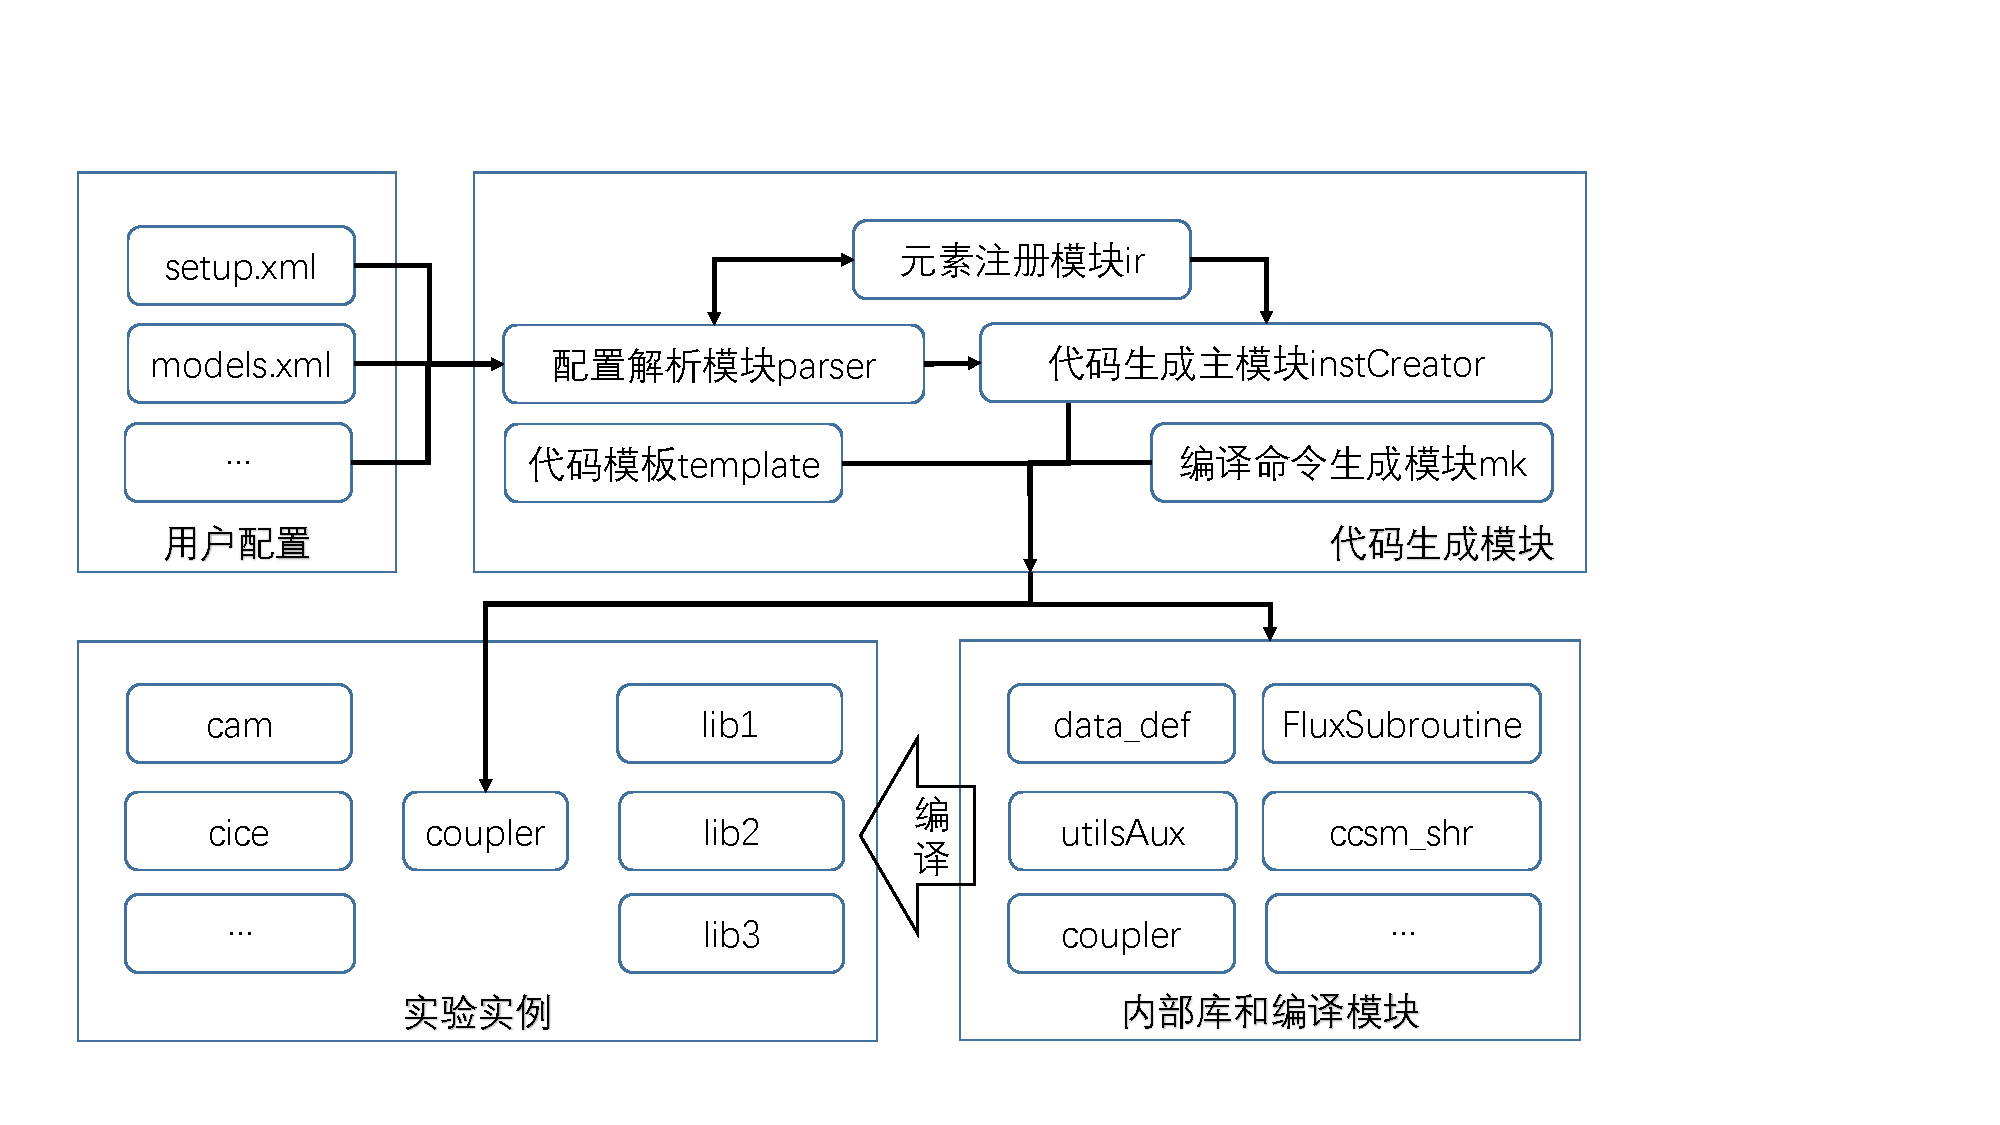
\includegraphics[width=1\textwidth]{../figures/fig1.pdf}
\caption{耦合平台运行流程图示例}
\end{figure}

\section{配置文件模块}

这部分是由用户提供的 xml 文件组成的配置集合。我们在适配各个模式分量实现的过程中对该部分的配置文件进行了规范化以降低用户配置的工作量和减少可能出现的错误配置和冗余导致的配置文件不一致。

在主要配置文件中,通过添加数据结构类型字段和网格比率类型字段,将不同类型的代码作为代码生成模块的内置函数自动生成,可以减少不同类型字段调用内部库函数时可能产生的冲突或错误。多个配置文件公用的分辨率、网格、接口类型等信息通过单独使用配置文件进行定义并通过短字符串代码进行引用的方式减少冗余和潜在的冲突或不一致可能。在配置文件中将各个模式分量独有的部分进行尽可能的隔离,并在共同接口处进行文件级引用,最大化各个模式分量实现的独立性,使得在将来多模式分量实现并行开发成为可能。简化了顶层耦合模块自身的配置文件,将部分相对固定的设置转移到编译选项和代码生成模块内部以精简配置文件和提高配置文件可读性。在外部文件引用模块中插入了默认的同网格映射配置,并在配置文件格式中区分了对内部不同数据结构可能存在的不同网格文件引用(虽然在目前用到的所有配置中这些文件都是相同的)以预备未来可能存在的高级设置。虽然我们目前的实验平台确定,我们还是提供了可配置的实验平台参数,该部分代码虽然未经过可扩展性测试,但在设计层面提供了原生跨平台的可能性。简化了伪模型的设计,省略了其与真模型相同但实质上无需配置的部分,使得对特定数据结构构造伪模型进行适配的时间成本一定程度上降低。将与物理过程相关的参数与代码实现相关的参数进行隔离,使得配置文件编写者可以专注于物理过程配置或代码层面配置。具体配置文件将会在下一章的实验结果中进行描述。

\section{代码生成模块}

这部分模块大部分为自动代码生成,对新加入的模式分量实现有较好的自动适配能力。这里主要是追加部分新功能和针对错误跟踪和调试进行结构上的修改。

\subsection{配置解析模块 parser}

该模块读入用户提供的 xml 配置文件并进行语法和语义检查,其中语法检查通过外部库来完成,而语义检查则通过内部自定义的 python 代码库完成。我们在调试模式开启时,将外部库的各个调用间插入了能够反映运行步骤的若干信息,从而可以在外部库发生错误的时候用代码生成模块内置的工具进行错误定位。在处理语义错误的情况时,我们通过与下面的元素注册模块配合以提前检查出部分冲突错误,并将可能的错误放在 ErrorHandler 模块下,通过多模块的协作将可能出现的错误在代码生成模块运行前即判明并尝试修复。另外,还修复了部分边界情况和空情况的处理,同时在这些情况下自动发出警告以避免配置文件编写错误。

\subsection{元素注册模块 ir}

由于部分模式分量自带一致性检测发现传输数据数量有误,追溯到配置解析模块发现耦合实验实例配置文件存在重复录入和局部名称冲突等问题。为了防止类似问题再次发生,在元素注册 ir 模块中加入了对各个数据域和跨模式分量的全局名称字典,在解析阶段即可进行全局冲突检测。这一步发生在代码生成之前,可以极大的节约编译运行和调试追溯时间。另外,针对部分很可能出现冲突的数据域,追加了可选用的顶层耦合内置前后缀的方式进行区分,降低了跨模式分量实现冲突可能。这一步操作需要内部库函数进行转译操作,且可能会导致在版本更新过程中带来的数据不一致问题,在最终进行数据分析时也要对外部工具进行修改,因此默认为关闭状态。

\subsection{代码生成主模块 instCreator}

这一部分本质上是通过 python 代码读取 xml 配置文件代码来生成 fortran 代码,这里需要大量的语义转换,最常见的就是 python 中的 True/False 和 fortran 中的 .true./.false. ,为了方便进行这些转换,我们在代码中添加了常见的翻译表,使得相同语义的不同语言表示可以在生成过程中自动切换。这在一定程度上减少编码复杂度,提高了代码可读性。需要注意的是这种语义自动转译需要配合转译字符使用,有较低概率会在用户编写特定文本时出现意料之外的转译,因此配合了日志模块和变异模块进行确认。

\subsection{编译命令生成模块 mk}

这部分可以通过耦合模式分量信息自动生成最终编译耦合实验主程序 coupler 的编译命令。通过各个模式分量自身的编译系统,所需的头文件和打包后的静态库文件被放置到设定的路径下,从而可以用相对路径找到。但对静态库的引用代码需要在编译命令生成模块中进行设置。为此,我们在输入的配置文件中加入了各个模式分量的输出命名规则,从而可以自动生成静态库链接代码,真正达成全自动生成和编译。

\section{内部库和编译模块}

这一部分的代码结构进行了调整,现在所有的 Makefile 进行了统一配置,其配置文件位于 baseCpl/src 目录下的 Makefile.conf 文件中,设置了 C++ 和 fortran 编译器及其主要依赖库的编译选项,包括 ESMF , NetCDF , ParallelIO 等外部库的头文件路径和库文件路径。与该模块相关的所有路径名称都要求设置为基于 ABSDIR 主目录宏的相对路径,这是为了在实验实例生成后路径变更时只需要对该宏进行自动修改即可在对应实例的目录下进行自动编译。各个依赖库的目录采用相对路径的方式对该配置文件进行引用,以确保在绝对路径改变后依然能够不依赖于宏地正确引用。

\subsection{数据定义模块 data\_def}

为了确保全局数据存储 global\_var 可以被多种模式分量实现用各自不同的方式进行访问和修改以提高适配面,降低适配难度,将所有分辨率修正前和修正后的数据结构对 MCT 的再封装进行展开,使得各个模式分量可以直接调用而不必通过顶层耦合模式进行解包,达成代码解耦的目的,同时也避免了多进程之间调用和多个模式分量实现之间可能存在的 race-condition 问题。

部分开关标记变量的副本转换为引用,牺牲少许效率换取原生的一致性。这一部分主要考虑到虽然顶层耦合模式存在多进程隔离的一致性保护,但各个模式分量实现编写过程中可能出现对这些变量的直接读取访问,这部分代码可能不受顶层耦合模式的隔离保护,因而可能会触发不一致的问题。值得一提的是,根据目前的框架和各个耦合模式分量的实现,并不存在将一个模式分量实现可写的数据暴露给另一个模式分量实现的情况,因此该设计仅为未来可能出现的该情况进行预先处理,在当前版本并未得到测试。

对通用宏进行了整合,现在默认字符串长度统一为 SHR\_KIND\_CS 和 SHR\_KIND\_CL 两个宏,这两个值在全局类型表文件 shr\_kind\_mod.F90 中被定义为所有不包含路径文本字符串的最大长度和全部文本字符串的最大长度,默认设为 80 和 256 个字符。在本修改前部分不带路径的文件名在 CESM 中被设定为 16 字符长度,因而出现了字符串溢出和命名冲突等问题。为此我们还插入了一个可选的字符串溢出检测模块,该模块开启时会对运行速度产生一定影响,但考虑到与字符串相关操作本身效率不高且已经被主要多进程运算部分尽可能避免,这部分实际测试中对运行效率的影响可以忽略不计,但仍然推荐在调试通过后的最终运行阶段关闭该模块。另外,我们对 CESM 中补充定义的 SHR\_KIND\_CX 和 SHR\_KIND\_CXX 两个宏进行了保留以方便其他模式分量的适配。这两个值预设为 512 和 4096。

\subsection{流数据传输模块 FluxSubroutine}

该模块用于不同模式分量实现中的数据传输时追加的适配数据处理。这部分代码涉及一定的物理运算,因此需要对调试工具进行适配从而可以检测出一个正确的模式分量输出在该模块由于数值溢出或误差等原因不满足目标模式分量输入的情况。另外,部分计算需要涉及到来自多个模式分量的多个数据结构,因此数据同步也要纳入错误检测范围内。实际上,在适配过程中出现了由于数据依赖关系复杂导致的运算顺序触发的错误,该错误在调试过程中无法被稳定复现,因此我们对该模块的调试模式加入了较强的同步要求以确保运行顺序不影响错误复现。

\subsection{输入合并模块 MrgSubroutine}

在加入新的模式分量实现后,需要根据其所需要的全部来自其他模式分量实现的数据编写输入合并模块,将这些数据整合进 run 模块的输入参数并进行必要的适配。考虑到各个模式分量对输入的处理存在较大差异,这部分代码没有采用代码生成模块自动进行生成而是要求用户自行编写。实际上,不共同模式分量实现的输入合并模块相似度很低,因此该设计并不增加各个模式分量适配的工作量,相反能够减少由于自动适配产生的接口冗余和可读性降低。与之相对的,该部分库函数代码所需的变量由代码生成模块处理并生成,使得人工编写该库函数时减少依赖变动。

\subsection{历史记录和存储恢复模块 utilsAux}

该模块调用 utils 进行文件读写,包括历史记录和存储恢复两部分。由于各个模块自身已有涉及这两个模块,且读写格式不统一,这里只处理顶层耦合模式可见的数据传输部分。来自各个模式分量的数据同名的情况通过插入来源模式分量名称进行区分,同时需要对后处理函数和数据分析工具进行调整。需要注意的是,经过顶层耦合模式的数据存在多种进程分配方式:按模式分量进程分配和按顶层耦合进程分配。他们所对应的全局分配表 GSMap 存在差异,需要用不同方式进行存储记录。这部分代码的更改主要是为了适配各种不同模式分量实现在数据存储上的不同情况而设置的多种输出过程。另外,为了使得顶层耦合模块可以正确输出模式分量实现自行配置的内容,需要在模式分量的 init 接口中对顶层耦合模块对应的数据接口配置文件进行设置,并由历史纪录和存储恢复模块进行读取以进行正确的对接和数据输出。

\subsection{CCSM 内置库模块 ccsm\_shr}

该模块存放了各个来源于 CCSM 的通用库函数,以备各个模式分量实现和顶层耦合模式中保留的来源于 CESM 的代码进行调用。由于该部分被完整地应用于 CESM 实际运行的实例中,因此正确性可以得到保证,但在我们适配的过程中可能会出现各种数据不匹配的情况,从而在调用正确的库函数过程中发生错误,从而定位到 ccsm\_shr 模块内部。因此,我们并不将这部分代码视作黑盒,而是在适当位置插入调试信息和数据追溯,以确保在该模块内部发生的异常可以较为容易的追溯到数据结构来源,从而达到提高调试效率的目的。同时,考虑到未来顶层耦合模式的更新对该模块进行可能的更改和再封装,又要和原版模式分量保持兼容性,我们对于重封装函数保留了原版接口。
